\documentclass{beamer}

% This file is a solution template for:

% - Talk at a conference/colloquium.
% - Talk length is about 20min.
% - Style is ornate.


\mode<presentation>
{
  \usetheme{Singapore}
  % or ...

  \setbeamercovered{transparent}
  % or whatever (possibly just delete it)
}


\usepackage[utf8]{inputenc}
\usepackage[english]{babel}
\usepackage{textcomp}

% \usepackage{times}
% \usepackage[T1]{fontenc}
% Or whatever. Note that the encoding and the font should match. If T1
% does not look nice, try deleting the line with the fontenc.

\usepackage{graphicx}
\usepackage{epstopdf}
\usepackage{amsmath}
\usepackage{amsfonts}
\usepackage{mathtools}
\usepackage{dsfont}
\usepackage{color}
\usepackage{verbatim}
\usepackage{tikz}
\usepackage{cite}

\title{Plasmonic Properties of QM 2D Fractals.}

\author{Tom Westerhout \\ 
        \emph{Supervisors:} Shengjun Yuan \& Edo van Veen \\
        TCM}
\date[BZ 2017]{Bachelor Zomersymposium, 2017}

\begin{document}

\begin{frame}
    \titlepage
\end{frame}

\section{Introduction}

\begin{frame}{Stained Glass}
    \begin{figure}
    \includegraphics[width=8cm]{stained-glass-bird}
    \end{figure}
\end{frame}

\begin{frame}{Plasmons}
    \begin{definition}[Plasmon]
        Quanta of plasma oscillation (\emph{think quasiparticle}).
    \end{definition}

    \begin{definition}[Plasma Oscillation]
        Longitudinal waves of electron charge-density.
    \end{definition}
\end{frame}

\begin{frame}{Simple example}
    \begin{itemize}
    \item<1-> Free electron gas with positively charged atom cores in the background.
    \item<1-> Oscillating electric field $\mathbf{E}(t) = \mathbf{E_0}\exp(-i\omega t)$.
    \item<2-> Equation of motion: \[ \mathbf{\ddot{x}} + \gamma\mathbf{\dot{x}} = -\frac{e}{m}\mathbf{E}(t)\; .\]
    \item<3-> Displaced electrons generate a polarization $\mathbf{P} = -Ne\mathbf{x}$ \\ ($N$ is the electron density).
    \item<4-> From $\epsilon_0\mathbf{E} + \mathbf{P} = \epsilon_0\varepsilon(\omega)\mathbf{E}$ \ we get $\varepsilon(\omega)$.
    \item<4-> In high frequency limit $\varepsilon(\omega) \approx 1 - \frac{\omega_p^2}{\omega^2}$, \\ $\omega_p$ --- \alert{plasma frequency}.
    \item<5-> If $\omega = \omega_p$, we get longitudinal oscillation of electron-charge density.
    \end{itemize}
\end{frame}

\begin{frame}{Fractals}
    \begin{itemize}
    \item Features: nowhere differentiable, have fractal dimensions, self-similar, etc.
    \item Ramification: minimum number of links that one needs to remove to separate a macroscopic part of infinite fractal.
        \begin{columns}[T]
        \column{0.6\textwidth}
            \emph{Finite ramification:} \alert{Solved analytically} \\ by L.P. Kadanoff (1982).
        \column{0.4\textwidth}
            \begin{figure}
            \input{Sierpinski-Gasket}
            \end{figure}
        \end{columns}

        \begin{columns}[T]
        \column{0.6\textwidth}
            \emph{Infinite ramification:} \alert{Unsolvable analytically} (?). Numerical calculations exist (\emph{done at Radboud}), but not of plasmonic properties.
        \column{0.4\textwidth}
            \begin{figure}
            \input{Sierpinski-Carpet}
            \end{figure}
        \end{columns}
    \end{itemize}
\end{frame}

\begin{frame}{Problem}
    \begin{itemize}
    \item Plasmonic properties are obtained from $\varepsilon$ \\
        $\implies$ \alert{Goal}: calculate $\varepsilon$.
    \item There exist good methods to calculate the dielectric function in \alert{momentum space}, i.e. rely on translational symmetry.
    \item In fractals, there is \alert{no translational symmetry}!
    \item Calculations have to be done in \alert{real space}. \\
        $\implies$ \alert{New method}.
    \end{itemize}
\end{frame}

\section{Method}

\subsection{RPA}

\begin{frame}{System}
    \begin{itemize}
    \item<1-> Electron system is described (in a one-particle approximation) by
        \begin{itemize}
        \item \alert{eigenenergies $\{E_i\}$} and
        \item \alert{eigenstates $\{|i\rangle\}$}.
        \end{itemize}
    \item<2-> Grand-canonical ensemble, i.e. \alert{temperature} $T$ and \alert{chemical potential} $\mu$ are fixed.
    \item<3-> Occupational numbers are given by the \alert{Fermi-Dirac distribution}
        \[ n_i = \frac{1}{\exp\!\left(\frac{E_i - \mu}{k_\text{B}\!T}\right) + 1} \;.\]
    \item<4-> Introduce a one-particle density matrix
        \[ \hat\rho_0 = \sum_i n_i\, |i\rangle\!\langle i| \;.\]
    \end{itemize}
\end{frame}

\begin{frame}{Random Phase Approximation}
    \begin{itemize}
    \item<1-> Perturbation of the form
        \[ \alert{\hat V e^{-i(\omega + i\eta)t}}\,,\text{ with }\eta \to +0\,. \]
        \small{($\hat V$ is diagonal in $\mathbf{r}$-basis, i.e. $\langle\mathbf{r}|\hat V|\mathbf{r'}\rangle = V(\mathbf{r})\delta^3(\mathbf{r} - \mathbf{r'})$)}
    \item<2-> Results in an induced charge density variation $\delta\hat N(t)$
    \item<3-> \alert{Self-consistency equation}
        \[ \langle \mathbf{r} | \hat V_\text{tot}(t) | \mathbf{r} \rangle
            = \langle \mathbf{r} | \hat V_\text{ext}(t) | \mathbf{r} \rangle + \int\!\! \text{d}^3 r' \; \langle \mathbf{r} | \hat V_\text{Coulomb} | \mathbf{r'} \rangle \langle \mathbf{r'} | \delta\hat N(t) | \mathbf{r'} \rangle \;. \]
    \end{itemize}
\end{frame}

\begin{frame}
    \dots a good excercise in calculus and Fourier analysis \dots
    \[ \implies \langle \mathbf{r} | \hat V_\text{ext}(\omega) | \mathbf{r} \rangle = \int\!\! \text{d}^3 r' \; \langle \mathbf{r} | \hat \varepsilon(\omega) | \mathbf{r'} \rangle \langle \mathbf{r'} | \hat V | \mathbf{r'} \rangle \; , \text{ where} 
    \]
    \vspace{-1.0cm}
    \begin{multline*}
        \begin{aligned}
        \langle \mathbf{r} | \hat \varepsilon(\omega) | \mathbf{r'} \rangle 
            &= \lim_{\eta \to 0+} \langle \mathbf{r} | \hat\varepsilon(\omega + i\eta) | \mathbf{r'} \rangle = \lim_{\eta \to 0+} \int\limits_{0}^{\infty} \!\! \text{d}\tau \; e^{i (\omega +i\eta) \tau}\,\langle \mathbf{r} | \hat\varepsilon(\tau) | \mathbf{r'} \rangle \\
            &= \langle \mathbf{r} | \mathbf{r'} \rangle - \lim_{\eta \to 0+} \sum_{i,\,j} \frac{n_i - n_j}{E_i \!-\! E_j - \hbar(\omega \!+\! i\eta)} \int\!\! \text{d}^3 r'' \frac{e^2}{\| \mathbf{r} - \mathbf{r''} \|}
        \end{aligned} \\
        \times \langle j |\mathbf{r''}\rangle \langle\mathbf{r''} | i \rangle \langle i | \mathbf{r'}\rangle \langle \mathbf{r'} | j \rangle
    \end{multline*}
\end{frame}

\begin{frame}{Tight Binding}
    \begin{itemize}
    \item<1-> Electrons are ``tightly bound'' to atoms \\
        $\implies$ \alert{atomic basis $\{|a\rangle\}$}
        \begin{itemize}
        \item $\langle a|b \rangle = \delta_{a,b}$ \hspace{0.5cm} and \hspace{0.5cm} $\sum_a |a\rangle \langle a | = \hat{\mathds{1}}$,
        \item $\langle \mathbf{r} | a \rangle \approx 1$.
        \end{itemize}
    \item<2-> Example Hamiltonian of the system is
        \[ \hat H = -t \,\sum_{\langle a, b \rangle} (\hat c_a^\dagger \hat c_b + \text{h.c.})\;,\]
        $\hat c^\dagger_a$ and $\hat c_a$ are creation and annihilation operators, $t$ is the \alert{hopping value}.
    \end{itemize}
\end{frame}

\subsection{Implementation}

\begin{frame}{Algorithm}
    Calculating $\hat\varepsilon$ for a single $\omega$ is an \alert{$\mathcal{O}(N^4)$ problem}, where $N$ is the number of particles.
    \begin{itemize}
    \item Hack: rewrite everything in terms of \alert{matrix operations} and use BLAS (\emph{Basic Linear Algebra Subroutines}).
    \item Use a \alert{supercomputer} for calculations.
    \item Hack: use \alert{symmetries} of the system.
    \end{itemize}
\end{frame}

\begin{frame}{Parallelisation}
    \begin{itemize}
    \item Use different cluster nodes (\emph{think small supercomputers}) to calculate $\hat\varepsilon$ for different frequencies \\
        $\implies$ \texttt{MPI}, \texttt{Boost}
    \item Use different threads to speed up matrix operations \\
        $\implies$ \texttt{Intel MKL}, \texttt{OpenMP}
    \end{itemize}
\end{frame}

\section{Results}

\subsection{Experiments}

\begin{frame}{Electron Energy Loss Spectroscopy (EELS)}
    \begin{itemize}
    \item<1-> Shoot electrons on the sample.
        \begin{itemize}
        \item<3-> Electron beam with a well-defined wavevector $\mathbf{k}$.
        \item<4-> Inelastic scattering results in \alert{energy loss $E = \hbar\omega$} and \alert{momentum transfer $\hbar\mathbf{q}$}.
        \end{itemize}
    \item<2-> Look at (usually) transmitted electrons.
        \uncover<5->{
        \[ \hspace{-2.5cm} \overbrace{\frac{\text{d}^2\sigma}{\text{d}\Omega\text{d}E}} ^\text{\normalsize double-differential cross section} \hspace{-2.0cm}\propto\; 
           \underbrace{-\operatorname{Im}\! \left[\frac{1}{\langle\mathbf{q}| \hat\varepsilon(\omega) |\mathbf{q}\rangle}\right]} _\text{\normalsize \alert{loss function}} \;.
        \] %
        }
    \end{itemize}
\end{frame}

\subsection{Calculations}

\begin{frame}{Third Iteration Sierpinski Carpet}{System}
    \begin{figure}
    \vspace{-.5cm}
    \input{Coordinates-SC-3}
    \end{figure}
\end{frame}

\begin{frame}{Third Iteration Sierpinski Carpet}{Results}
    \begin{figure}
    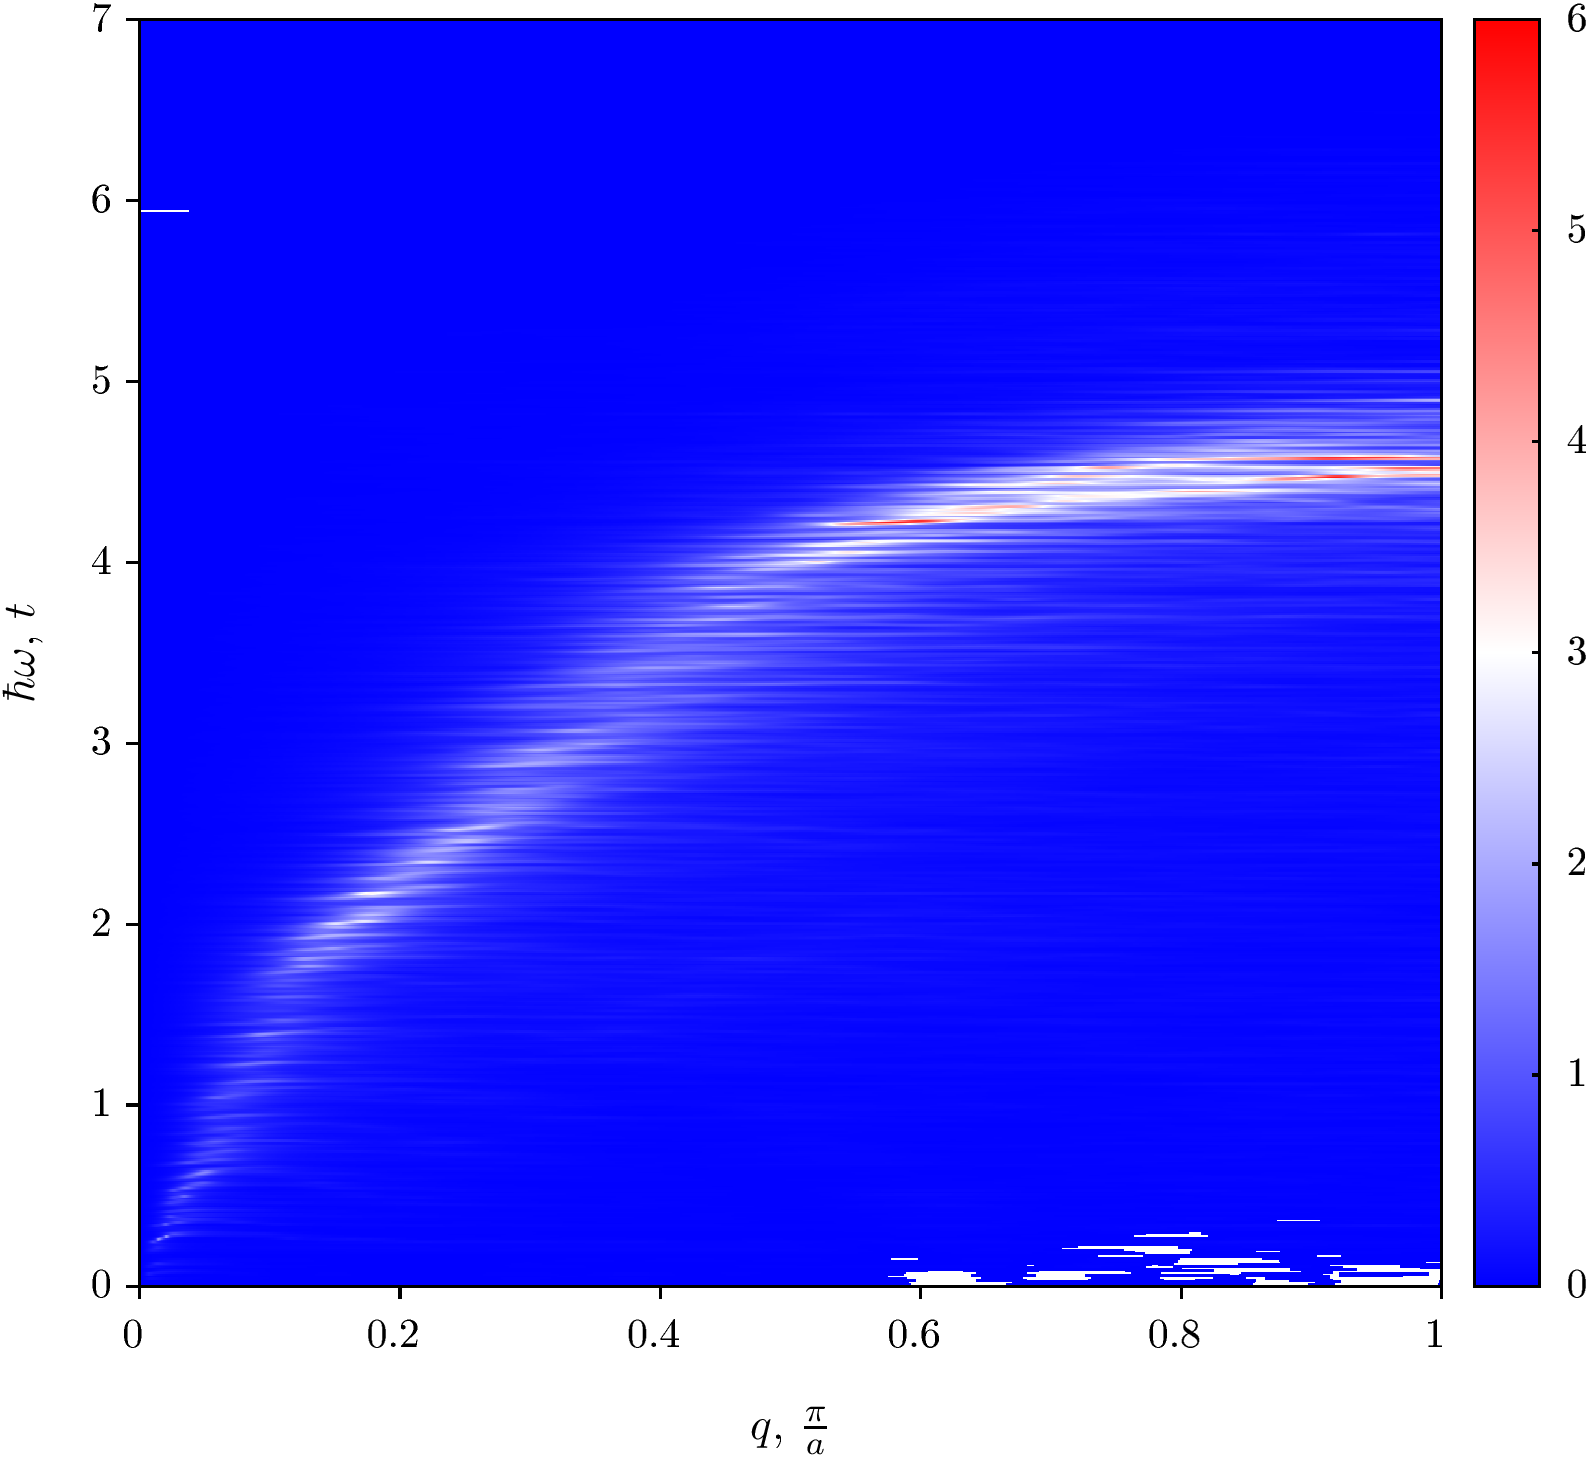
\includegraphics{Spectrum-3rd-Q-Omega}
    \end{figure}
\end{frame}

\begin{frame}{Square Lattice}{Results}
    \begin{figure}
    \includegraphics{Spectrum-3rd-SL-Q-Omega}
    \end{figure}
\end{frame}



\section*{Summary}

\begin{frame}{Summary}
  \begin{itemize}
  \item \Large{It \emph{is} possible to do calculations of $\hat\varepsilon$ in real space.}
  \item \Large{There \emph{are} well defined plasmons in Sierpinski carpets.}
  \end{itemize}
\end{frame}

\begin{frame}{}
    \vfill
    \begin{minipage}{\textwidth}
    \begin{center}
        \Large Any questions?
    \end{center}
    \end{minipage}
    \vfill
\end{frame}


% All of the following is optional and typically not needed. 
\appendix
\section<presentation>*{\appendixname}
\subsection<presentation>*{For Further Reading}


\end{document}



